\documentclass[]{article}
\usepackage{amssymb}
\usepackage{amsmath}
\usepackage{amsthm}
\newtheorem{lemma}{Lemma}
\newtheorem{corollary}{Corollary}
\newtheorem{proposition}{Proposition}
\newtheorem{theorem}{Theorem}
\theoremstyle{definition}
\newtheorem{definition}{Definition}
\theoremstyle{remark}
\newtheorem{remark}{Remark}
\newcommand{\lemmaautorefname}{Lemma}
\usepackage[utf8]{inputenc}
\usepackage{amsmath}
\usepackage{amsfonts}
\usepackage{array}
\usepackage[hidelinks]{hyperref}
\usepackage[english]{babel}
\usepackage{float}
\newcommand{\enstq}[2]{\left\{#1\mathrel{}\middle|\mathrel{}#2\right\}}
\newcommand{\norm}[1]{\left\|#1\right\|}
\newcommand{\N}{\mathbb{N}}
\newcommand{\Z}{\mathbb{Z}}
\newcommand{\D}{\mathbb{D}}
\newcommand{\R}{\mathbb{R}}
\newcommand{\duality}[2]{\left\langle #1,#2\right\rangle}
\newcommand{\inner}[2]{\left( #1,#2\right)}
\newcommand{\abs}[1]{\left\lvert #1 \right\rvert}
\newcommand{\toDo}[1]{{\color{red}#1}}
\newcommand{\Cinf}{C^{\infty}}
\newcommand{\isdef}{\mathrel{\mathop:}=}
\newcommand{\opFromTo}[3]{#1 : #2 \longrightarrow #3}
\usepackage{todonotes}
\usepackage{subcaption}
\DeclareMathOperator{\DL}{\textup{DL}}
\DeclareMathOperator{\W}{\textup{W}}
\DeclareMathOperator{\curl}{\mathbf{curl}} 
\let\div\undefined
\DeclareMathOperator{\div}{\textup{div}} 
\makeatletter
\newsavebox{\@brx}
\newcommand{\llangle}[1][]{\savebox{\@brx}{\(\m@th{#1\langle}\)}%
	\mathopen{\copy\@brx\kern-0.5\wd\@brx\usebox{\@brx}}}
\newcommand{\rrangle}[1][]{\savebox{\@brx}{\(\m@th{#1\rangle}\)}%
	\mathclose{\copy\@brx\kern-0.5\wd\@brx\usebox{\@brx}}}
\makeatother
\newcommand{\dduality}[2]{\llangle#1\,, #2\rrangle}
\usepackage{todonotes}
\usepackage{subcaption}
\makeatletter    
\renewcommand*{\vec}[1]{\boldsymbol{#1}}
\makeatother

\title{Sign conventions for the Nédélec and Raviart-Thomas elements in Gypsilab}
\author{}


\begin{document}
\maketitle


\section{Surfacic spaces}

\subsection*{Notation}


A triangular mesh $\mathcal{M}$ is given by a set of vertices 
$$\mathcal{V} = \enstq{v_i \in \R^3}{i \in \{1,\ldots,N_\mathcal{V}\}}$$ 
and a set of elements 
$$\mathcal{T} = \enstq{t_l \in \N^3}{l = 1\ldots,N_{\mathcal{T}}}\,.$$

The element $t_l = (i,j,k)$ encodes the triangle given by the vertices $v_i$, $v_j$ and $v_k$. Note that this provides an orientation to the triange: $(i,j,k)$ is not the same triangle as $(i,k,j)$, for example. We assume that the mesh is conforming, in the sense that the intersection of two closed triangles in $\mathcal{M}$ is either empty, a common vertex or a common edge. 
We denote by $\Gamma$ the union of the closed triangles in $\mathcal{T}$. We furthermore assume that $\Gamma = \partial \Omega$ where $\Omega$ is a Lipschitz domain. 


\begin{itemize}
	\item A call to V $= \mathcal{M}$.vtx returns an $N_{\mathcal{V}} \times 3$ array, such that V(i,:) is the row vector $v_i$. 
	\item A call to T $= \mathcal{M}$.elt returns an $N_{elt} \times 3$ array such that T$(l,:)$ is the row vector $t_l$. 
\end{itemize}


The set of edges $\mathcal{E}$ of $\mathcal{M}$ is the set 
\[\mathcal{E} = \enstq{1 \leq i < j \leq N_{\mathcal{V}}}{v_i \textup{ and } v_j \textup{ are vertices of a common triange}}\,.\]
The edges are arbitrarily ordered as $\mathcal{E} = \{e_1, \ldots, e_{N_\mathcal{E}}\}$. 
\begin{itemize}
	\item A call to `edg2vtx = $\mathcal{M}$.edg.elt' returns a $N_{\mathcal{E}} \times 2$ array such that ${\textup{edg2vtx}(m,:)}$ is the row vector $e_m$. 
\end{itemize}

The meshes that we deal with are supposed to be {\bf well-oriented}, in the sense that for any two triangles $t = (i,j,k)$ and $t' = (i',j',k')$, the sets
\[ \{(i,j), (j,k), (k,i)\} \textup{ and } \{(i',j'), (j',k'), (k',i')\}\]
are {\bf mutually disjoint}. In other words, if two triangles $t$ and $t'$ share an edge $(i,j)$ then the indices $i$ and $j$ must appear in a different order in $t$ and $t'$, e.g.
$t = (i,j,k)$ and $t' = (j,k',i)$. 
The unit normal vector of the triangle $t = (i,j,k)$ is defined by 
$$\vec n_t = \frac{\overrightarrow{v_iv_j} \times \overrightarrow{v_iv_k}}{\norm{\overrightarrow{v_iv_j} \times \overrightarrow{v_iv_k}}}\,.$$
Normal vectors of the triangles of $\mathcal{M}$ are accessed through Nrm = $\mathcal{M}$.nrm. Then, Nrm(l,:) is the row vectors of the coordinates of $\vec n_t$ where $t = t_l$. 
The fact that the mesh is well-oriented implies that for two neighboring triangles, the orientation of the normal is consistent\footnote{For $t$ and $t'$ sharing the edge $e$, on can rotate $t'$ about the axis $e$ such that the two triangles are in the same plane and do not overlap. The orientation of the normal is consistent if the normal vector of the rotated triangle $t'$ is equal to the normal vector of $t$. }. 

The edge normal vectors of $t = (i,j,k)$ are defined by 
$$\vec \nu_{l}( v_i) \isdef \frac{\overrightarrow{v_jv_k} \times \vec n_t}{\norm{\overrightarrow{v_jv_k} \times \vec n_t}}\,, \quad \vec \nu_{l}( v_j) \isdef \frac{\overrightarrow{v_kv_i} \times \vec n_t}{\norm{\overrightarrow{v_kv_i} \times \vec n_t}}\,, \quad \vec \nu_{l}( v_k) = \frac{\overrightarrow{v_iv_j} \times \vec n_t}{\norm{\overrightarrow{v_iv_j} \times \vec n_t}}\,.$$
They point outward of the triangle $t$. Those vectors are accessed through the call 
\[\textup{NrmEdg}= \mathcal{M}.\textup{nrmEdg}\,,\] 
then NrmEdg\{i\}(l,:) is the row vector of the coordinates of $\vec \nu_{i,l}$ 

\begin{figure}[H]
	\centering
	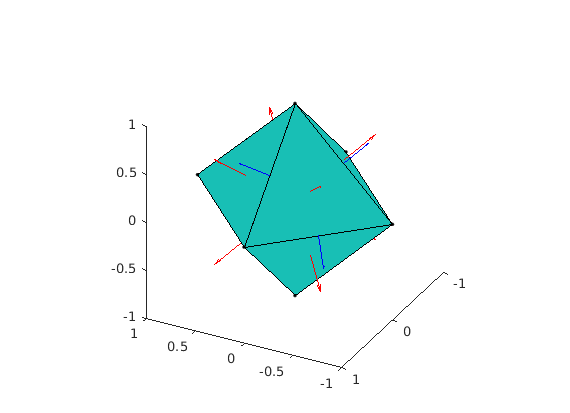
\includegraphics[width=0.4\textwidth]{mshExample}
	\caption{Example of mesh, with normal vectors represented in red, and the edge normals represented in blue for the frontmost triangle.}
\end{figure}

\subsection*{Raviart-Thomas elements}

The Raviart-Thomas space obtained by calling the function `fem($\mathcal{M}$,``RWG")'\footnote{In Gypsilab, Raviart-Thomas elements are referred to as Rao-Wilton and Glisson elements \cite{rao}.} is
\[\textup{Span}\enstq{\vec{\phi}_e}{e \in \mathcal{E}}\]
where for an edge $e = (i,j)$ (with $i < j$), $\vec \phi_e$ is defined as follows. On a triangle $t$ that doesn't have the edge $e$, $\vec \phi_e = 0$. On the other hand, if $x \in t$ where $t$ has the edge $e$, then
\[\vec \phi_e(x) \isdef s\frac{\overrightarrow{v_k x}}{2\mathcal{A}(t)}\]
where $\mathcal{A}(t)$ is the area of $t$, $\vec v_k$ is the third vertex of $\mathcal{T}$ and $s$ is equal to $1$ if $(i,j,k)$ and $t$ are equal up to a circular permutation, and $-1$ otherwise.
The fact that $\mathcal{M}$ is well-oriented implies that $\vec\phi_e$ is in $H(\div,\Omega)$. The flux of $\vec \phi_e$ through the edge $e$ verifies
\[\int_{e} \vec \phi_e \cdot \vec \nu_k \,d\sigma_e = s\,.\]

\subsection*{Nédélec elements}

The Nédélec finite element space obtained by calling the function `fem($\mathcal{M}$,``NED")' is 
\[\textup{Span}\enstq{\vec{\psi}_e}{e \in \mathcal{E}}\]
where for an edge $e = (i,j)$, $\vec \psi_e$ is defined as follows. On a triangle $t$ that doesn't have the edge $e$, $\vec \phi_e = 0$. On the other hand, if $x \in t$ where $t$ has the edge $e$, then $\vec \psi_e(x)$ is the vector orthogonal to $\vec n_t$ such that
\[ \vec \psi_e \isdef -\vec n_t \times \vec\phi_e \iff \vec n_t \times \vec \psi_e(x) = \vec \phi_e(x)\]
where $\vec \phi_e$ is defined above. It is thus clear that the operator `$\vec n_t \times \cdot$' maps the Nédélec to the Raviart-Thomas bijectively. Define $\vec \tau_e \isdef \frac{\overrightarrow{v_iv_j}}{\norm{\overrightarrow{v_iv_j}}}$. Then the circulation of $\vec \psi_e$ on $e$ verifies
\[\int_{e} \vec \tau_e \cdot \vec \psi_e d\sigma_e= - \int_{e} [\vec n_t, \vec \phi_e,\vec \tau_e]d\sigma_e \]
where $[\vec a,\vec b,\vec c] = \vec a \cdot (\vec b \times \vec c)$. If $t_l$ and $(i,j,k)$ are equal up to a circular permutation, then $\vec \nu_l(v_k) = \vec \tau_e \times \vec n_t$, so  
\[\int_{e} \vec \tau_e \cdot \vec \psi_e d\sigma_e = -\int_e \vec \phi_e \cdot \vec n_t = -s = -1\]
On the other hand, if $(i,j,k)$ and $t_l$ are not equal up to circular permutation, then $\vec \tau_e \times \vec n_t = -\vec \nu_l(v_k)$ and again
\[\int_{e} \vec \tau_e \cdot \vec \psi_e d\sigma_e = \int_e \vec \phi_e \cdot \vec n_t = s = -1\,.\]
It would probably be a bit more natural to define the Nédélec element and the Raviart-Thomas basis functions as the opposite of what is currently done in Gypsilab, but what really matters is to be aware of the sign convention and be consistent with it. 


\section{Volumetric spaces}

\subsection*{Tetrahedral meshes}

Tetrahedral meshes are just like triangular meshes, except the elements are tetrahedrons, encoded by $4$-uples of indices. The tetrahedrons must be {\textbf{well-oriented}}, in the sense that if $(i,j,k,l)$ encodes a tetrahedron, then the determinant
\[[\overrightarrow{v_iv_j},\overrightarrow{v_iv_k},\overrightarrow{v_iv_l}]\]
must be \textbf{negative}. 
The normal vector of a tetrahedron does not make sense, nor do the edge normal. However, one can define the face normals. If $\vartheta = (i,j,k,l)$ is a tetrahedron, its (oriented) faces are 
\[t_1 = (j,k,l) \,\,,\,\, t_2 = (k,l,i)\,\,,\,\, t_3 = (l,i,j)\,\,,\,\,t_4 = (i,j,k)\,.\] 
The normal vectors are given by $\vec n_{t_i}$ $i = 1\ldots 4$ as defined for triangles. The fact that a tetrahedron is well-oriented implies that the face normal vectors point outwards of the tetrahedron $\vartheta$. 


\subsection*{Raviart-Thomas elements}

Now the Raviart-Thomas space is the Span of vector field $\vec \phi_t$ associated to the faces $t$ of the mesh. Each face can be shared by at most $2$ elements. Consider a face $t$ given by the vertices are $v_i,v_j,v_k$ sorted such that $i < j < k$. Let $\vartheta$ be a tetrahedron possessing the face $f$, and let $\vec n_t$ be the normal vector to the face pointing out of $\vartheta$. Then the function $\vec \phi_t$ is defined on $\vartheta$ by 
\[\vec \phi_t(\vec x) = s\frac{\vec x - \vec v_0}{3\mathcal{V}(\vartheta)}\]
where $\mathcal{V}(\vartheta)$ is the volume of the tetrahedron, $v_0$ is the fourth vertex of $\vartheta$ and 
\[s = - \textup{sign}(\overrightarrow{v_i v_j}\times \vec n_t)\,.\]
Once again, we are surprised by the sign convention in Gypsilab but it doesn't matter as long as we know it. 

\begin{thebibliography}{0}
	\bibitem{rao}
	Rao, S. M., Wilton, D. R. and Glisson, A. W.:
	\newblock Electromagnetic scattering by surfaces of arbitrary shape 
	\newblock {\em IEEE. Trans. Antennas and Propagation} 30(3), 409--418 (1982)
\end{thebibliography}

\end{document}
